\documentclass{article}

\usepackage{lipsum}
\usepackage[margin=1.2in]{geometry}
\usepackage{titlesec}
\usepackage{graphicx}

\newcommand{\code}{\texttt}

% Specify images directory
\graphicspath{ {./report-images/} }

% Header and Footer stuff
\usepackage{fancyhdr}
\pagestyle{fancy}
\fancyhead{}
\fancyfoot{}
\fancyfoot[R]{ \thepage\ }
\renewcommand{\headrulewidth}{0pt}
\renewcommand{\footrulewidth}{0pt}
\newcommand{\sectionbreak}{\clearpage}
\setlength{\parindent}{0pt}

%

\begin{document}

%----------------------------------------------------------------------------------------
%	TITLE PAGE
%----------------------------------------------------------------------------------------

\begin{titlepage} % Suppresses displaying the page number on the title page and the subsequent page counts as page 1
	\newcommand{\HRule}{\rule{\linewidth}{0.5mm}}% Defines a new command for horizontal lines, change thickness here
	
	\center % Centre everything on the page
	
	%------------------------------------------------
	%	Headings
	%------------------------------------------------
	
	\textsc{\Large Data Fitting}\\[0.5cm] % Major heading such as course name
	
	\textsc{\large Exercise 3}\\[0.5cm] % Minor heading such as course title
	
	%------------------------------------------------
	%	Title
	%------------------------------------------------
	
	\HRule\\[0.6cm]
	
	{\huge\bfseries Comparison between Polynomial and Natural Cubic Spline Interpolation}\\[0.25cm] % Title of your document
	
	\HRule\\[1.5cm]
	
	%------------------------------------------------
	%	Author(s)
	%------------------------------------------------
	
	\begin{minipage}{0.4\textwidth}
		\begin{flushleft}
			\large
			\textit{Author}\\
			\textsc{Cesare De Cal} % Your name
		\end{flushleft}
	\end{minipage}
	~
	\begin{minipage}{0.4\textwidth}
		\begin{flushright}
			\large
			\textit{Professor}\\
			\textsc{Annie Cuyt}\\ % Supervisor's name
			[0.25cm]
			\textit{Assistant Professor}\\
			\textsc{Ferre Knaepkens} % Supervisor's name

		\end{flushright}
	\end{minipage}
	
	% If you don't want a supervisor, uncomment the two lines below and comment the code above
	%{\large\textit{Author}}\\
	%John \textsc{Smith} % Your name
	
	%------------------------------------------------
	%	Date
	%------------------------------------------------
	
	\vfill\vfill\vfill % Position the date 3/4 down the remaining page
	
	{\large\today} % Date, change the \today to a set date if you want to be precise
	
	%------------------------------------------------
	%	Logo
	%------------------------------------------------
	
	%\vfill\vfill
	%\includegraphics[width=0.2\textwidth]{placeholder.jpg}\\[1cm] % Include a department/university logo - this will require the graphicx package
	 
	%----------------------------------------------------------------------------------------
	
	\vfill % Push the date up 1/4 of the remaining page
	
\end{titlepage}

%----------------------------------------------------------------------------------------

\section{Introduction}\label{sec:intro}
An imaginary chemistry experiment produces the following data set:

  \begin{table}[!ht]
    \large        %% not "\fontsize{12}{12}\selectfont"
    \centering    %% not "\center{...}"
    \begin{tabular}{|c|c|c|c|c|c|c|c|}
    \hline
    \it{x}\textsubscript{i}&-1&-0.96&-0.86&-0.79&0.22&0.50&0.93\\     %% no "&" at start of row
    \it{f}\textsubscript{i}&-1.000&-0.151&0.894&0.986&0.895&0.500&-0.306\\
    \hline        %% extra \hline at bottom of table
    \end{tabular}
  \end{table}

The purpose of this exercise is to use these data points to compute and plot the interpolating polynomial together with the natural cubic spline, and to report what it is observed. My hypothesis is that there may be an unsatisfactory oscillating behavior in the polynomial interpolant, whereas the natural cubic spline will be stiffer with less tendency to oscillate because it is a piece-wise type of interpolation. 

\section{Tools}
The following programming language and libraries have been used in this exercise:
\begin{itemize}
  \item Python 3.7
  \item SciPy
\end{itemize}
The SciPy \code{interpolate} sub-package was used to compute the interpolating polynomial and the natural cubic spline:
\begin{itemize}
  \item \code{scipy.interpolate.lagrange(x, y)}
  \item \code{scipy.interpolate.CubicSpline(x, y, bc\_type)}
\end{itemize}

The following NumPy methods of the SciPy environment have been used in this exercise:
\begin{itemize}
  \item \code{numpy.array(object)}
  \item \code{numpy.linspace(start, stop, num)}
  \item \code{numpy.polynomial.polynomial.Polynomial(poly)}
  \item \code{numpy.setprint\_options(precision)}
  \end{itemize}
The following Matplotlib methods of the SciPy environment have been used in this exercise to plot:
 \begin{itemize}
  \item \code{matplotlib.pyplot.plot(x, y, formatting, label)}
  \item \code{matplotlib.pyplot.legend()}
  \item \code{matplotlib.pyplot.show()}
  \item \code{matplotlib.pyplot.figure(dpi)}
  \item \code{matplotlib.pyplot.ylim(miny, maxy)}
  \item \code{matplotlib.pyplot.xlabel(name)}
  \item \code{matplotlib.pyplot.ylabel(name)}
  \end{itemize}
  
\section{Computation and plotting}
The exercise asks to compute the interpolating polynomial of the given data set. To do so, I first create two arrays in Python containing the data points using \code{np.array} and a linear space from -1 to 1 containing 1000 points. These values are finally passed to the \code{lagrange} method which returns the {\it Lagrange} interpolating polynomial (\code{poly = lagrange(x, y)}). \\

The following are coefficients the interpolating polynomial retrieved with \code{Polynomial(poly).coef}:
 \begin{itemize}
  \item 4.3649939020826437e-02
  \item 1.6076695441034385e+01
  \item -4.8402059220598259e-02
  \item -2.0100476671430044e+01
  \item 1.6880653327119008e-02
  \item 5.0294636999940936e+00
  \item -6.4460635283115466e-03
  \end{itemize}
  
The polynomial of the 6th degree in the {\it power} form is: \\

$0.04365005085x^6 + 16.0766955610565x^5 - 0.048402197837630x^4 - 20.10047681678335740x^3\\ + 0.0168806991536721320x^2 + 5.029463735952404423200x - 0.006446071786954468800$ \\

In order to calculate the natural cubic spline I use the built-in SciPy method \code{CubicSpline(x, y, bc\_type)} and use "Natural" for the \code{bc\_type}. The coefficients are the following:\\

$[[-8.0654538905002710e+02  1.4844899135604635e+02  2.5130673577722442e+02
  -7.2398801257531864e-01  1.2138819568393451e+00  5.0415317855085340e-01]
 [-8.5265128291212022e-14 -9.6785446686003496e+01 -5.2250749279189527e+01
   5.2366523402757015e-01 -1.6700184440756460e+00 -6.5035760033060053e-01]
 [ 2.2515472622480029e+01  1.8644054755039885e+01  3.7404351585205808e+00
   1.1953927535924665e-01 -1.0382774667893093e+00 -1.6879827592230572e+00]
 [-1.0000000000000000e+00 -1.5100000000000000e-01  8.9400000000000002e-01
   9.8599999999999999e-01  8.9500000000000002e-01  5.0000000000000000e-01]]$

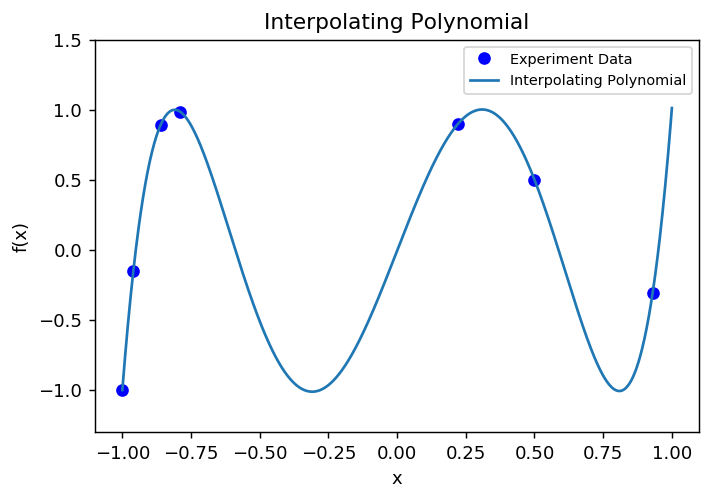
\includegraphics[width=\textwidth,height=\textheight,keepaspectratio]{lagrange.png}
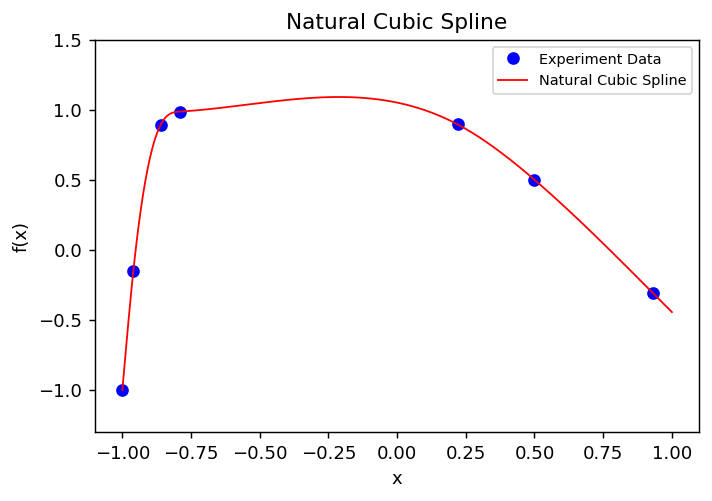
\includegraphics[width=\textwidth,height=\textheight,keepaspectratio]{nspline.png}
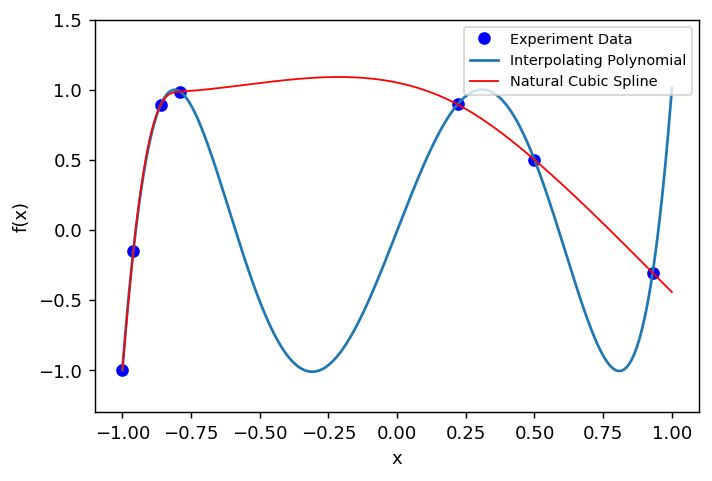
\includegraphics[width=\textwidth,height=\textheight,keepaspectratio]{together.png}

\section{Observations}
The natural cubic spline is a much more accurate representation than the {\it Lagrange} function which appears inconsistent with several {\it ups and downs}.\\

Since the natural cubic spline is a type of piece-wise interpolation, the graph passes through the experiment data points with low-degree polynomials. Since we only use low-degree polynomials, we eliminate the excessive oscillations that are present in the interpolating polynomial.

\end{document}